\documentclass[tikz,border=2pt]{standalone}
\usepackage{times}
\usepackage{amsmath,amssymb}
\begin{document}
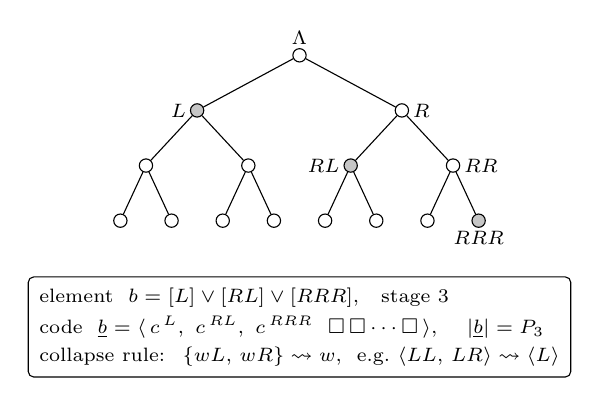
\begin{tikzpicture}[
  font=\scriptsize, level distance=7mm,
  level 1/.style={sibling distance=26mm},
  level 2/.style={sibling distance=13mm},
  level 3/.style={sibling distance=6.5mm},
  every node/.style={inner sep=1.2pt},
  sel/.style={circle, draw, fill=gray!45, inner sep=1.7pt},
  unsel/.style={circle, draw, inner sep=1.7pt}
]
\node[unsel, label=above:{$\Lambda$}] {}
  child { node[sel, label=left:{$L$}] {}
    child { node[unsel] {} child { node[unsel]{} } child { node[unsel]{} } }
    child { node[unsel] {} child { node[unsel]{} } child { node[unsel]{} } } }
  child { node[unsel, label=right:{$R$}] {}
    child { node[sel, label=left:{$RL$}] {}
      child { node[unsel]{} } child { node[unsel]{} } }
    child { node[unsel, label=right:{$RR$}] {}
      child { node[unsel]{} } child { node[sel, label=below:{$RRR$}]{} } } };
\node[draw, rounded corners=2pt, align=left, inner sep=4pt, font=\scriptsize] at (0,-3.45) {
  element \ $b=[L]\vee[RL]\vee[RRR]$,\quad stage $3$\\[2pt]
  code \ $\underline b=\langle\, c^{\,L},\ c^{\,RL},\ c^{\,RRR}\ \ \square\,\square\cdots\square\,\rangle$, \quad $|\underline b| = P_3$\\[2pt]
  collapse rule: \ $\{wL,\,wR\}\rightsquigarrow w$, \ e.g.\ $\langle LL,\, LR\rangle \rightsquigarrow \langle L\rangle$
};
\end{tikzpicture}
\end{document}
